\documentclass[a4paper,12pt]{article}
\usepackage[utf8x]{inputenc}
\usepackage[swedish]{babel}
\usepackage[T1]{fontenc}
\usepackage{graphicx}
\usepackage{subcaption}
\usepackage{placeins}
\usepackage{amsfonts, amsmath, amssymb}
\usepackage{ccfonts,euler}
\usepackage{wrapfig}
\usepackage{multirow}
\usepackage{caption}
\usepackage{enumerate}
\usepackage{comment}
\usepackage[includeheadfoot,margin=1.1in]{geometry}
\usepackage{hyperref}
\usepackage{listings}
\usepackage{color}

\definecolor{dkgreen}{rgb}{0,0.6,0}
\definecolor{gray}{rgb}{0.5,0.5,0.5}
\definecolor{mauve}{rgb}{0.58,0,0.82}

\lstset{frame=tb,
  language=Python,
  aboveskip=3mm,
  belowskip=3mm,
  showstringspaces=false,
  columns=flexible,
  basicstyle={\small\ttfamily},
  numbers=none,
  numberstyle=\tiny\color{gray},
  keywordstyle=\color{blue},
  commentstyle=\color{dkgreen},
  stringstyle=\color{mauve},
  escapeinside={\%*}{*)},
  breaklines=true,
  breakatwhitespace=true,
  tabsize=3,
  literate={å}{{\r a}}1 {ö}{{\"o}}1 {ä}{{\"a}}1 {Å}{{\r A}}1 {Ö}{{\"O}}1 {Ä}{{\"A}}1
}

\oddsidemargin -15mm
\evensidemargin -15mm
\marginparwidth 5mm
\topmargin -28mm
\textheight 282mm
\textwidth 190mm
\headheight 4mm
\headsep 4mm

\sloppy

\newcounter{iii}\setcounter{iii}{0}
\def\i{\bigskip\noindent\refstepcounter{iii}\textbf{\arabic{iii}.} }
%\def\iotst#1{\par \smallskip \mbox{}\refstepcounter{iii}\hspace*{#1}\textbf{\arabic{iii}.}}
\newcounter{pun}[iii]
\def\pu{\refstepcounter{pun}{\bf(\alph{pun})}\ }
\def\Pu{\par\noindent\mbox{}\refstepcounter{pun}{\phantom{\textbf{\arabic{iii}.}}\hspace{0.2mm}\bf(\alph{pun})}\ }

\def\ext{\subsection*{Extrauppgifter}}

\title{Programmering, Nao - Pass 5}
\date{2 augusti}

\makeatletter
\let\newtitle\@title
\let\newdate\@date
\makeatother
\begin{document}

  \renewcommand*\rmdefault{ppl}\normalfont\upshape
\pagestyle{empty}
\large
\section*{\newdate\ \  \newtitle}

\i \textbf{Talföljden}

Att fortsätta en påbörjad talföljd är en vanlig sorts uppgift i såväl matteböcker som IQ-tester. Men det smartaste måste väl ändå vara att skriva ett datorprogram som löser problemet en gång för alla.

Betrakta till exempel de så kallade triangeltalen:

1, 3, 6, 10, 15, 21 . . .

Ett mönster framträder om man tittar på skillnaden mellan varje tal och dess föregångare:

2, 3, 4, 5, 6 . . .

Tydligen ökar skillnaden med 1 i varje steg. Men för någon annan talföljd kan skillnaden till exempel öka med 13, minska med 2 eller vara konstant. Det enda som är säkert om de talföljder som förekommer i denna uppgift är att skillnaden mellan två intill varandra stående tal ändras lika mycket i varje steg.

Skriv ett program som frågar efter de tre första talen i talföljden (positiva heltal mindre än 100) och sedan skriver ut de 10 första talen åtskilda med blanksteg.

\textbf{Körningsexempel:}
\begin{lstlisting}
Första talet ? 1
Andra talet ? 3
Tredje talet ? 6
Talföljden: [1, 3, 6, 10, 15, 21, 28, 36, 45, 55]
\end{lstlisting}

\begin{comment}
print("Skriv de 3 första talen i talföljden")
tal1 = int(input("Första talet: ")) #får in de 3 första talen i talföljden
tal2 = int(input("Andra talet: "))
tal3= int(input("Tredje talet: "))

skillnad1 = tal2-tal1 #tar ut skillnaden mellan de 2 första talen
skillnad2 = tal3-tal2 # tar ut skillnaden mellan tal 2 och tal 3

skillnad = skillnad2 - skillnad1 #jämför de 2 skillnaderna för att se hur mycket skillnaden ökar

temp_skillnad = skillnad2 #temporär skillnad. Skillnaden mellan varje enskilt tal
#Här väljer man antingen att skriva en lista (enklare) eller en string med alla svar (Det är detta uppgiften frågar om)
tal = [tal1, tal2, tal3] #För att skapa lista (med komma och hakparantes)
string = "%s %s %s"%(tal1, tal2, tal3) #för att skapa en string med mellanrum
for i in range(3,10):
    # Ser på talet innan i talföljden och adderar skillnaden mellan de 2 talen innan samt adderar skillnaden mellan alla skillnader
    tal.append(tal[i-1]+skillnad+temp_skillnad)
    string += " %s" %(tal[i-1]+skillnad+temp_skillnad)
    temp_skillnad += skillnad #ökar skillnaden mellan 2 tal allt eftersom
#Skriver ut en lista eller en string med tal, beroende på vad man valt att göra.
print(tal)
print(string)
\end{comment}

\i \textbf{Snöskottning}

Scott har som många andra haft problem under vintertiden med allt snö. Scotts hus måste skottas ofta, men han tycker själv att skotta varje dag är för ofta. Du ska hjälpa Scott att sätta upp ett skott-schema för de kommande N dagarna. Till din hjälp har du en detaljerad väderleksprognos, så du vet exakt hur många cm det snöar eller smälter varje dag (innan kvällen). När det ligger minst H cm snö en kväll så är det dags att skotta, och när man skottar så försvinner all snö. Från början är det ingen snö alls.

\textbf{Indata}

Första raden innehåller antalet dagar $1 \le N \le 100$ och andra raden snötröskeln $1 \le H \le 1000$. Därefter följer N heltal mellan $-100$ och $100$ (inklusive). Dessa tal beskriver hur många cm snö det kommer under var och en av de kommande N dagarna. Ett negativt värde betyder att denna mängd smälter istället (men snötäcket kan naturligtvis aldrig bli mindre än 0).

\textbf{Utdata}

Utdatat ska bestå av ett heltal, antalet kvällar Scott måste skotta.

\textbf{Körningsexempel:}
\begin{lstlisting}
Antal dagar? 10
Snögräns? 27
Snöförändringar? 5 -7 8 19 -20 22 8 26 -15 14
Scott behöver skotta minst 2 gånger
\end{lstlisting}


\begin{comment}
N = 10 #Antalet dagar, 1<=N<=100
H = 27 #snötröskel - när det är så här många cm snö MÅSTE det skottas, 1<=H<=1000

#snöförändring - ett heltal mellan -100 och 100 (inklusive). Negativt värde = smälter, positivt värde = snöar
snoforandring = [5, -7, 8, 19, -20, 22, 8, 26, -15, 14]

sno_pa_marken = 0 #Uppdaterar snön på marken varje dag
antal_skottningar = 0 #Uppdaterar antal skottningar som måste göras
for i in range(N):
    sno_pa_marken += snoforandring[i] #lägger till snön som kom över natten till gårdagens snö
    if sno_pa_marken >= H: #kollar om snön är över/lika med max-gränsen
        sno_pa_marken = 0 #nollställer isf snön (all snö är bortskottad)
        antal_skottningar += 1 #lägger till att vi har skottat en gång
    if sno_pa_marken < 0: #kollar om det finns möjlighet att smälta mer snö än det finns
        sno_pa_marken = 0 #nollställer isf snön (så det inte kan vara negativ snö)
        
print("Scott behöver skotta minst ", antal_skottningar, " gånger.")
\end{comment}
\i \textbf{Kölappar}

Du råkar gå till banken i rusningstid. Ett vanligt kölapps-system används, men $n$ kunder har lägre könummer än du. Dock är $m$ kassor öppna. Skriv ett program som, givet hur lång tid varje kunds ärende tar, beräknar hur lång tid det tar innan det är din tur.

Varje kund har ett bankärende som tar ett helt antal minuter. Så fort det finns en ledig kassa kallas nästa person i kön fram. Kundbytet tar inget tid i anspråk. För enkelhets skull förutsätter vi att i det ögonblicket du tar din kölapp, låt oss kalla det tiden 0, så är alla kassorna lediga och m kunder kallas alltså fram omedelbart (vilket kan inkludera dig om $n < m$).

\textbf{Indata}

Programmet tar emot antalet personer före dig i kön ($1 \le n \le 100$) och antalet öppna kassor ($1 \le m \le 10$). Därefter följer en rad med $n$ heltal i intervallet 1..20, antalet minuter för varje kunds ärende. 

\textbf{Utdata}
Programmet ska skriva ut efter hur många minuter du kallas fram och får påbörja ditt ärende.


\textbf{Körningsexempel:}
\begin{lstlisting}
Antal kunder ? 7
Antal kassor ? 3
Tid för varje kund ? 2 5 6 2 4 5 3
Du kallas fram efter 8 minuter.
\end{lstlisting}

\begin{comment}
n = 7 #antal kunder före dig i kön, 1<=n<=100
m = 3 #antal kassor öppna, 1<=m<=10

tid_för_varje_kund = [2, 5, 6, 2, 4, 5, 3] #lista över antalet minuter det tar per kund

from numpy import zeros
kassor = zeros(m) #skapar en array (lista) där alla elementen är 0, med lika många element som antalet kassor

for i in range(n):
    kassor.sort() #sorterar så att kassan med minst total tid kommer först
    kassor[0] += tid_för_varje_kund[i] #lägger till en ny person i kassan som blir klar fortast
kassor.sort() #sorterar den en sista gång för att se vilken kö som är kortast när vi står först i kön
print("Väntetid: ",kassor[0], " minuter") # Vi tar kön med kortast tid av dessa.

\end{comment}


\i \textbf{Soldater}

\begin{figure}[!ht]
\centering
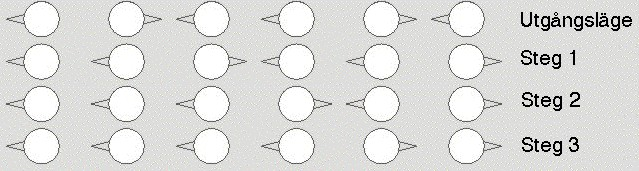
\includegraphics[width=0.8\textwidth]{soldater.jpg}
\caption{Uppställning av soldater}
\label{fig:soldater}
\end{figure}

Ett antal soldater står på ett led alla vända mot furiren, när han ger ordern "höger om". Eftersom många av soldaterna har svårt att skilja på höger och vänster blir det mest slumpen som avgör åt vilket håll de vänder sig. Ett exempel visas på första raden i figuren ovan. De soldater som på så sätt hamnar ''öga mot öga'' med en granne förstår båda två att de vänt sig åt fel håll och gör därför helt om (180 grader), för att kanske hamna öga mot öga med den andra grannen. Denna procedur fortsätter (steg 1 och 2 i figuren) och upphör då inga soldater längre är vända mot varandra (steg 3).

\textbf{Indata}

En rad där varje tecken är antingen V eller H. Dessa anger åt vilket håll soldatens näsa pekar i utgångsläget. Maximalt 100 tecken. 

\textbf{Utdata}
Programmet ska skriva ut hur många steg som behövs från utgångsläget tills lugnet infinner sig.

\textbf{Körningsexempel:}
\begin{lstlisting}
Soldater? VHVVHV
Det behövs totalt 3 steg för att lugna soldaterna

Soldater? HVHVHVHHVHVHVHVVHHHHVHHVHVVVHHVHHVHVHVHVHVHVHHH
Det behövs totalt 24 steg för att lugna soldaterna
\end{lstlisting}

\begin{comment}
persons = input("Soldater? ")
count = 0 # antalet vändningar
while "HV" in persons: # så länge minst två soldater står bredvid varandra
    persons = persons.replace("HV", "VH") #vänd soldaterna
    count += 1
print(count)
\end{comment}

\begin{comment}
-------------------------------------------------------------------
\end{comment}

\i \textbf{Tågväxeln}

Innan gymnasiet öppnades i Lillerud fanns endast en tågstation på den här platsen. Nu är dock både tågstation och räls borta sedan länge. 

Tågstationens föreståndare, Loke, hade jobbat där i många år. Hans jobb gick ut på att styra stationens manuella tågväxel. Det fanns bara två tåglinjer, antingen till Karlstad eller till Grums. Tågen gick periodiskt med $m$ respektive $n$ minuters mellanrum på de två linjerna, med första avgång $m$ respektive $n$ minuter efter midnatt. Alla tåg åkte alltså ut från stationen åt samma håll men delades sedan upp på två olika spår med hjälp av en växel. 

Loke fick lön baserat på hur många gånger han måste ändra växeln på en dag. Arbetsgivaren undrade hur många gånger som Loke måste ändra på växeln under ett helt dygn (dvs 1440 minuter). Tågen avgår alltså bara under minuterna 00:00 till 23:59.

Loke skulle ändra växeln enligt reglerna:
\begin{enumerate}
\item Om ett tåg ska avgå, och växeln är fel inställd, måste Loke ändra växeln till rätt spår.
\item Om båda tåg ska avgå samma minut, så avgår först det tåg som växeln är inställd för, och sedan ska Loke ändra växeln till det andra tågets spår.
\end{enumerate}

I början var växeln inställd på spåret för det tåg som avgår först.

Skriv ett program som beräknar hur många gånger som Loke måste ändra växeln under ett helt dygn.

\textbf{Körningsexempel}
\begin{lstlisting}
Talet m ? 450
Talet n ? 180
Antal växlingar: 5

Talet m ? 500
Talet n ? 1000
Antal växlingar: 1

Talet m ? 719
Talet n ? 720
Antal växlingar: 2

Talet m ? 7
Talet n ? 4
Antal växlingar: 410
\end{lstlisting}

\begin{comment}
print("Tågen går med m respektive n minuters mellanrum.")
m = int(input("Talet m = ")) #Ena tåget avgår var m-te minut
n = int(input("Talet n = ")) #Andra tåget avgår var n-te minut

N = 1440 # antal minuter på ett dygn


antal_vaxelandringar = 0 #Räknar antalet gånger Loke måste växla
for minuter in range(N): #Räknar fram till minut 1440 (0-1439, minut 1440 ej påbörjad)
    if minuter == 0:
        if m>n: #Spåret börjar på den sidan vars tåg åker iväg först. Behover darfor inte vaxla spar.
            spak = "n"
        else:
            spak = "m"
    elif minuter%m == 0 and minuter%n == 0: #kollar om båda tågen avgår från stationen samtidigt
        if spak == "m": #Tåget vars spår redan är växlad rätt kör först, därefter växlar Loke och det andra tåget kan köra iväg
            spak = "n"
            antal_vaxelandringar += 1
        else:
            spak = "m"
            antal_vaxelandringar += 1
    elif minuter%m == 0: #Om enbart det ena tåget är vid stationen
        if spak != "m": #kollar om det är nödvändigt att växla
            spak = "m"
            antal_vaxelandringar += 1
    elif minuter%n == 0: #Om enbart det andra tåget är vid stationen
        if spak != "n": #kollar om det är nödvändigt att växla
            spak = "n"
            antal_vaxelandringar += 1

print("Antal växlingar: ", antal_vaxelandringar)

\end{comment}

\pagebreak

\i \textbf{Robotar}

Fredrik gillar skattjakter, jättemycket. Och robotar, faktiskt ännu mer. Nu har han programmerat en robot att följa en skattkarta. 

På skattkartan är varje ruta markerad med pilar för att visa åt vilket håll roboten ska gå från den rutan.

Roboten börjar alltid i den ruta som befinner sig längst upp till vänster på skattkartan, och följer därefter pilarna. I labyrinten finns det två olika mål: ett batteri, samt en läskig elstöt. Det kan också hända att skattkartan leder runt roboten i en oändlig cykel av rutor så den aldrig når ett mål.

Kan du hjälpa roboten att avgöra vilket mål den når, eller om den kommer gå runt i all oändlighet.

\textbf{Indata}
Följande tecken förekommer i skattkartan:
\begin{itemize}
\item ''<'' – ruta med vänsterpil,
\item ''>'' – ruta med högerpil,
\item ''v'' – ruta med nedåtpil,
\item ''\^{}'' – ruta med uppåtpil,
\item ''B'' – rutan batteriet befinner sig på,
\item ''E'' – rutan elstöten befinner sig på.
\end{itemize}
Roboten börjar på den första rutan i den första raden av skattkartan. Skattkartan är konstruerad så att roboten aldrig kommer lämna labyrinten när den följer pilarna.

\textbf{Utdata}

Ditt program ska skriva ut vad som händer för roboten. 

\textbf{Körningsexempel:}
\begin{lstlisting}
vB<
vE^
>>^
Roboten kommer gå till Batteriet.
v>>v
>^Ev
vv^v
B<^<
Roboten får en elstöt.
v<E
>^B
>>^
Roboten kommer gå runt, runt, runt för evigt. 
vv<<<<<
vv>>v^^
vv^<vB<
vE^v<<^
v>^v^<^
>^<>>>^
Roboten kommer gå till Batteriet. 
\end{lstlisting}

\begin{comment}
karta = []
# Läser in kartan
while True:
    rad = input()
    if not rad:
        break
    karta.append(list(rad))


# Börjar simuleringen
x = 0
y = 0
while True:
    if karta[y][x] == 'B':
        print("Roboten kommer gå till Batteriet")
        break
    if karta[y][x] == 'E':
        print("Roboten kommer få en Elstöt")
        break
    if karta[y][x] == 'X':
        print("Roboten kommer gå runt, runt, runt för evigt")
        break

    # Eftersom vi skriver över värdet i kartan så sparar vi undan det först
    # Så vi kan minnas var vi ska förflytta oss i kartan
    riktning = karta[y][x]
     # Sätt rutan till besökt
    karta[y][x] = 'X'
    
    if riktning == 'v':
        y+=1
    elif riktning == '^':
        y-=1
    elif riktning == '<':
        x-=1
    elif riktning == '>':
        x+=1

\end{comment}




\i \textbf{Travar med böcker}

\begin{figure}[!ht]
\centering
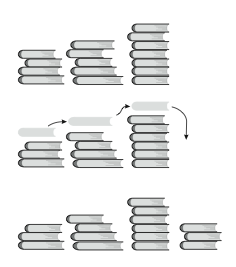
\includegraphics[width=0.3\textwidth]{Travar}
\caption{Första dagen plockas en bok från var och en av de tre travarna. Dessa tre böcker bildar en ny trave till höger om de andra.}
\label{fig:bocker}
\end{figure}

På ett bord ligger att antal travar med böcker. Varje dag tas en bok från varje trave. Dessa böcker bildar tillsammans en ny trave till höger om de andra, se figur~\ref{fig:bocker}. Om en trave blir tom skjuts travarna samman från höger. Eftersom det finns ett ändligt antal böcker, kommer förr eller senare samma upplägg att återkomma. Din uppgift blir nu att skriva ett program som frågar efter första uppläggets utseende och sedan tar reda på hur lång tid det tar innan ett upplägg som tidigare funnits, återkommer.

\begin{center}
  \begin{tabular}{ l | c | c | c | c | c | c }
Dag	& Hög 1 & Hög 2	& Hög 3	& Hög 4	& Hög 5	& Hög 6 \\ \hline
1	&4	&5	&7	&   &   &	 \\
2	&3	&4	&6	&3	&   &	 \\
3	&2	&3	&5	&2	&4  &	 \\
4	&1	&2	&4	&1	&3	&5   \\
5	&1	&3	&2	&4	&6	&    \\
6	&2	&1	&3	&5	&5	&    \\
7	&1	&2	&4	&4	&5	&    \\
8	&1	&3	&3	&4	&5	&    \\
9	&2	&2	&3	&4	&5	&    \\
10	&1	&1	&2	&3	&4	&5   \\
11	&1	&2	&3	&4	&6	&    \\
12	&1	&2	&3	&5	&5	&    \\
13	&1	&2	&4	&4	&5  &    \\
  \end{tabular}
\end{center}


I tabellen ovan visas hur antalet böcker i travarna varierar under 13 dagar. I de kommande testerna är antalet böcker $\le50$, antalet travar som mest $\le15$ och antalet dagar $\le100$.

\textbf{Körningsexempel (motsvarande tabellen ovan):}
\begin{lstlisting}
Antal travar ? 3
Böcker i trave 1 ? 4
Böcker i trave 2 ? 5
Böcker i trave 3 ? 7
Dag 13 uppkom ett upplägg, som redan förekommit dag 7
\end{lstlisting}

\begin{comment}
antal = int(input("Antal travar ? "))
travar = []
for i in range(antal):
    travar.append(int(input("Böcker i trave "+ str(i+1) + "?")))

history = []

def seen_before(travar):
    for trave in history:
        if trave == travar:
            return True
    history.append(travar[:])
    return False

while not seen_before(travar):
    antal = 0
    i = 0
    while i  < len(travar):
        if travar[i] > 0:
            travar[i] -= 1
            antal += 1
        if travar[i] == 0:
            del travar[i]
        else:
            i += 1
    travar.append(antal)
    #print(travar)

print("Dag",len(history)+1,"uppkom ett upplägg som redan funnits förut")
\end{comment}

\i \textbf{Trubaduren}

I en by på landet sjunger byborna varje kväll visor vid brasan. En viktig bybo är trubaduren. De kvällar trubaduren är närvarande sjunger han en ny visa som ingen annan bybo hört förut. Inga andra visor sjungs dessa kvällar, och alla bybor som då är närvarande lär sig trubadurens nya visa. De kvällar trubaduren inte är närvarande så sjunger byborna utan honom, och utbyter alla visor de kan med varandra.

Givet vilka bybor som är närvarade vid ett visst antal kvällar, skriv ut en lista på de bybor som efter dessa kvällar känner till samtliga visor som sjungits under den perioden.

\textbf{Indata}

Första raden innehåller heltalet N ($1 \le N \le 100$), antalet personer i byn, inklusive trubaduren. Byborna numreras från 1 till $N$, där bybo nummer 1 är trubaduren. Andra raden innehåller heltalet $M (1 \le M \le 50)$, antalet kvällar det sjungs visor i byn. Därefter följer $M$ rader som beskriver vilka bybor som närvarat de olika kvällarna. Ingen bybo kommer nämnas mer än en gång per rad, och trubaduren kommer att närvara åtminstone en kväll.

\textbf{Utdata}

Skriv ut de bybor, inklusive trubaduren, som kan alla olika visor som sjungits efter de $M$ kvällarna. 

\textbf{Körningsexempel}
\begin{lstlisting}
Antal personer? 6
Antal dagar? 5
Dag 1? 1 3
Dag 2? 2 3 4
Dag 3? 2 1 5
Dag 4? 2 4
Dag 5? 5 6
Svar: 1 2 4

Antal personer? 5
Antal dagar? 7
Dag 1? 1 2 4
Dag 2? 3 4 5
Dag 3? 1 2 3 4
Dag 4? 1 3 4 5
Dag 5? 3 4
Dag 6? 2 3 4 5
Dag 7? 1 3 5
Svar: 1 3 5
\end{lstlisting}

\begin{comment}
-------------------------------------------------------------------
\end{comment}

\end{document}
